% !TEX root = /Users/Gela/Desktop/Thesis_latex/thesis.tex
\section{Overview Method}
The working method during the thesis have been based on model based design in which a model and a physical system have been built in parallel.\\ 
\\
First, studies of theory and on previous work in the field were made in order to investigate requirements. After that, a flow chart investigation and test planning were made in parallel. Thereafter, modelling in Simscape and the construction of the first test rig, a rig using only one  pump,  was done. Afterwards, the one pump system was tested and the data from all the sensors were gathered.\\
\\
Analysis of the data was made and the rig was modified with two pumps to simulate the proposed two pump system. This was done in parallel with the modelling of the two pump system. \\
\\
After the tests on both systems were completed, an extensive comparison of the two systems were made. In figure \ref{fig:metod} an overview of the work flow can be seen to get a better overview.\\
\\
The data gathered from the tests could then be used to design an optimal control algorithm. 

\begin{figure}[h]
    \centering
    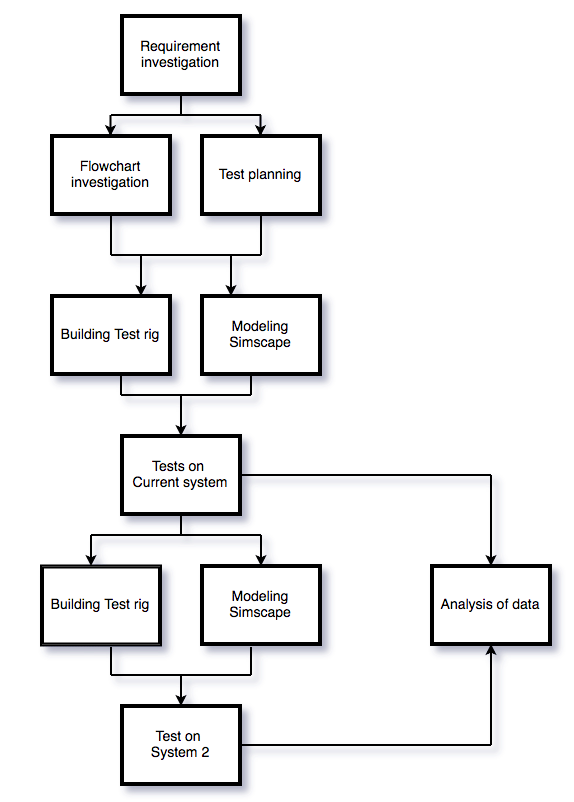
\includegraphics[width=0.8\textwidth]{Metod}
    \caption{Overview of method}
    \label{fig:metod}
\end{figure}\newpage




\section{Modeling}
The Simscape software tool described in section Appendix A is used to do a physical system model in order to model the characteristics of the membrane. The isolated system with pump, pipes, valves and water supply (tank) is implemented. The matematical equations used in the simulation can be seen in chapter \ref{sec:doweq}. The temperature correction factor, $TCF$ is implemented with equation \ref{eq:TCF} to simulate the temperature dependency of the membrane. The osmotic pressure, $P_{osm}$ is implemented in the model by equation \ref{eq:feedOsmP}. The polarization factor, $P_{f}$ that describes the polarization along the membrane surface is implemented with equation \ref{eq:polfac}. 
\\
\\
Dimensions on valves and pipes are implemented as the dimensions in the water device. Water quality, and temperature can be adjusted to simulate different conductivity and temperatures, to represent real values. The pump speed can be adjusted in the model to represent an actual value. Plots of characteristics of pressure, flow, salt concentration and temperature are generated from the simulations and can be seen in section \ref{sec:modres}

\section{Flowchart investigation}
\label{Flowchart}
Today, a system containing one pump is used by Baxter. The pump is positioned at the feed side of the membrane. The pump creates a pressure to overcome the osmotic pressure and creates a flow from feed to permeate side. The system can be seen in figure \ref{fig:System11}. The pump is used at two different set points on speed depending of the water quality (conductivity). There are no control implemented to adjust the speed (besides these two set points) of the pump in order to create different pressure and flow characteristics over the membrane to increase performance due to these different conditions. The valve in the recirculation path is adjusted when installing the water device at the clients and is not adjustable after that, other than by a service technician.\\
\\
\begin{figure}[h]
    \centering
    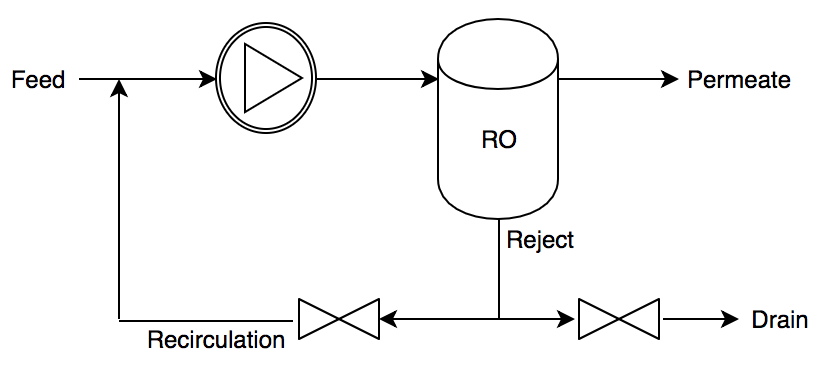
\includegraphics[width=0.5\textwidth]{Sys1}
    \caption{One pump system}
    \label{fig:System11}
\end{figure}

This limits the possibility for the water device to adapt itself to different working conditions and changes in inlet water quality and also if the membrane surface is fouling. Overcoming these issues would enable the water device to adapt to seasonal variations and changing temperature and tap water quality. If the membrane performance could be improved in all conditions and especially when the conditions vary over time the freedom of controlling the pumps and valve is desirable to optimize the performance of the membrane. \\
\\
To be able to investigate the performance and the feasibility of replacing the one pump system with a two pump system in order to control the flow and pressure over the membrane two different ideas were considered. Desirable outputs for increasing the membrane performance are:\\
\\
\begin{enumerate}
\item Pressure drop over the membrane is high
\item Flow through membrane is high
\end{enumerate}
The expected results of an optimization is that: the permeate conductivity is minimized, fouling on the membrane surface is minimized, the temperature dependencies is taken care of, waste water is minimized and the energy efficiency of the system is increased. In this thesis the investigations are limited to:\\
\\
\begin{enumerate}
\item Permeate conductivity is kept under 30 \SI{}{\micro\siemens}
\item The temperature dependencies are handled with control asystem
\item Waste water is minimized
\item Energy efficiency is improved compared to current one pump solution
\end{enumerate}
Different system setups were considered to implement the second pump. The two most promising ideas are presented below.

\subsection{System 1}
The first system has one pump on the feed side and one pump on the permeate side, as seen in figure \ref{fig:FlowCInves1}. This setup contributes with the ability to create a greater net pressure over the membrane with a low, or even a negative gauge pressure on permeate side, while the feed pump creates a high pressure on feed side. Benefits with this implementation is the low energy consumption due to the ability to create negative pressure on the permeate side. A high net driving pressure (pressure difference from feed to permeate side) can be achieved with rather low pressure on the feed side. The disadvantage might be that the second pump may contaminate the permeate stream. 

\begin{figure}[H]
    \centering
    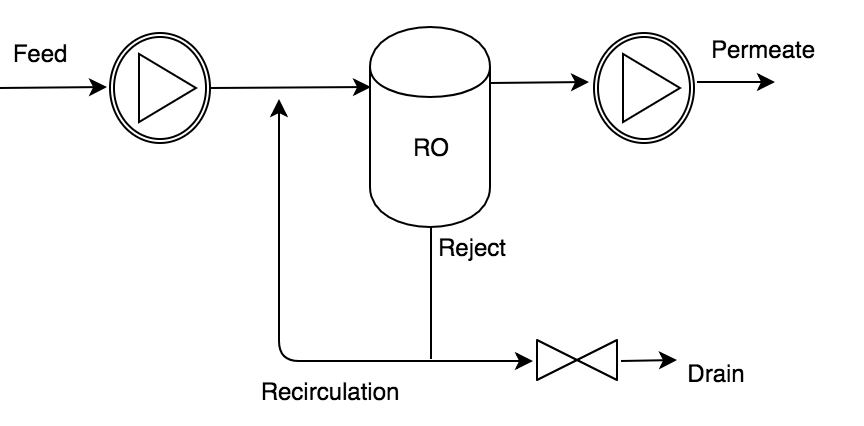
\includegraphics[width=0.7\textwidth]{FlowCInves1}
    \caption{System 1}
    \label{fig:FlowCInves1}
\end{figure}

\subsection{System 2}
The second system considered has one pump on the feed side and one pump in the recirculation loop, as seen in figure \ref{fig:Sys2}. The feed pump is used to create high pressure on the feed side and the pump in the recirculation path is used to control the flow in the recirculation path. As a result, the recovery rate can be controlled. According to theory the membrane behaviour is dependent on feed and flow characteristics over the membrane, salt concentration and temperature. \\
\\
\begin{figure}[H]
    \centering
    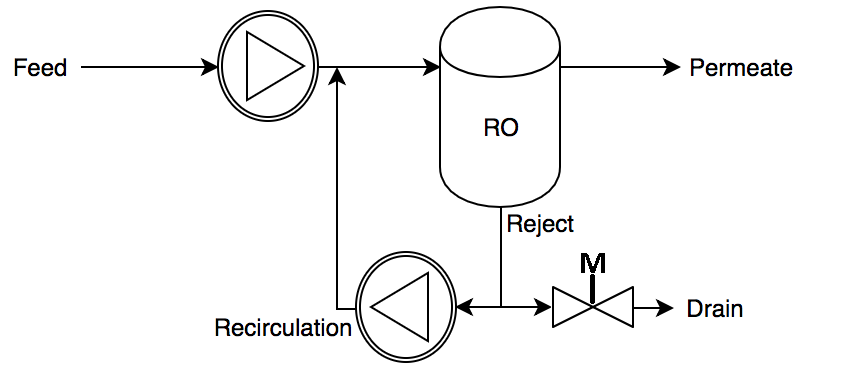
\includegraphics[width=0.7\textwidth]{Sys2}
    \caption{System 2}
    \label{fig:Sys2}
\end{figure}
Both system 1 and system 2 enables the ability to control pressure and recirculation flow independently.However, one big disadvantage with system 1 is that one of the pumps is positioned on the  permeate side and this could potentially contaminate the permeate. System 1 was therefore precluded.

\section{Flow measurements using the pumps}
In order to investigate the performance of the membrane, the pressure, flow, conductivity and temperature are measured and logged. The test rig should be able to operate at 15 bar and this made it difficult to find sensors that were able to function at such high pressure. The solution was to build our own sensor blocks and to use the feedback from the hall sensors in the pumps to measure the flow. \\
\\
Due to lack of instruments that could measure the flow under the high pressure some mapping of the flow from the pumps was made. The flow stream through the pumps were measured at different RPMs and with different pressure resistance on the outlet. The flow is depending on the RPM with negligible difference depending on the applied outlet pressure from the pump. The results from the mapping can be seen in the results chapter. 

\section{Implementation Test Rig}
\subsection{Current System}
In order to run all tests a physical rig was built. A first version was built to simulate the system used today, see figure \ref{fig:MeasCurrSys}, with all the measurement sensors implemented. The first version of the rig contained one pump with power supply, one RO-membrane, three needle valves, one drain valve, one heating bath, three measurement sensors, pipes and couplings. The heating bath is used to simulate different inlet water temperatures. The needle valves are used to adjust the pressure in the system to correspond with the real pressure characteristic in the water device. \\
\\
In order to log all signals and to run the system on the Real-Time Target Machine described in Appendix A is connected with all significant signals. A GUI designed in Simulink to control the rig is also connected to the rig. All control and feedback signals to and from the rig is handled in Simulink. After a test all measurements could be downloaded to a computer for analysis. Selected signals and calculations could also be displayed on a separate screen in real-time. \\
\\
\begin{figure}[H]
    \centering
    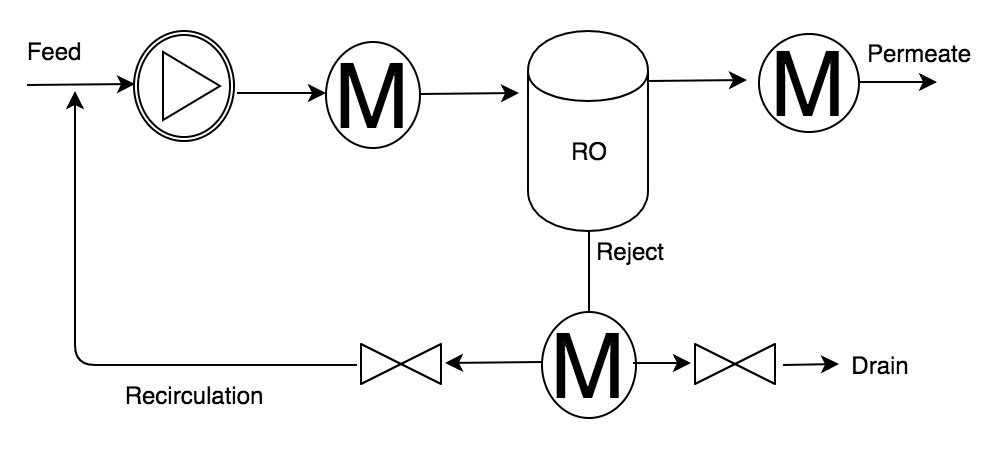
\includegraphics[width=0.7\textwidth]{MeasCurrSys}
    \caption{Current System, with measurement sensors}
    \label{fig:MeasCurrSys}
\end{figure}

\subsection{System 2}
The second system, System 2, was built by modifying the first rig, according to figure \ref{fig:MeasSys2}. The second rig contains: two pumps with power supply, one RO-membrane, three needle valves, one drain valve, one heating bath, one flow meter, three measurement sensors, pipes and couplings. The heating bath is used to simulate different inlet water temperatures. The needle valves are used to adjust the pressure in the system to correspond with the real pressure characteristic in the water device. The flow meter is used to measure the permeate flow from the membrane. \\
\\
The Simulink workspace, and the GUI was modified to be able to log all signals from the rig. All signals are displayed in real time as in the previous rig edition. Data is sampled and logged to be able to analyse the behaviour in the two pump system.  \\
\\
Different interfaces, as $i^{2}c$, Analog I/O, Digital inputs, PWM were used to implement the communication between the Real-Time Target Machine and measurement instruments. Circuits were built to transform voltage supply to required level for each component. All implementation of the communication and power supply can be seen in Figure \ref{fig:PressConn} - \ref{fig:PumpConn}. 

\begin{figure}[H]
    \centering
    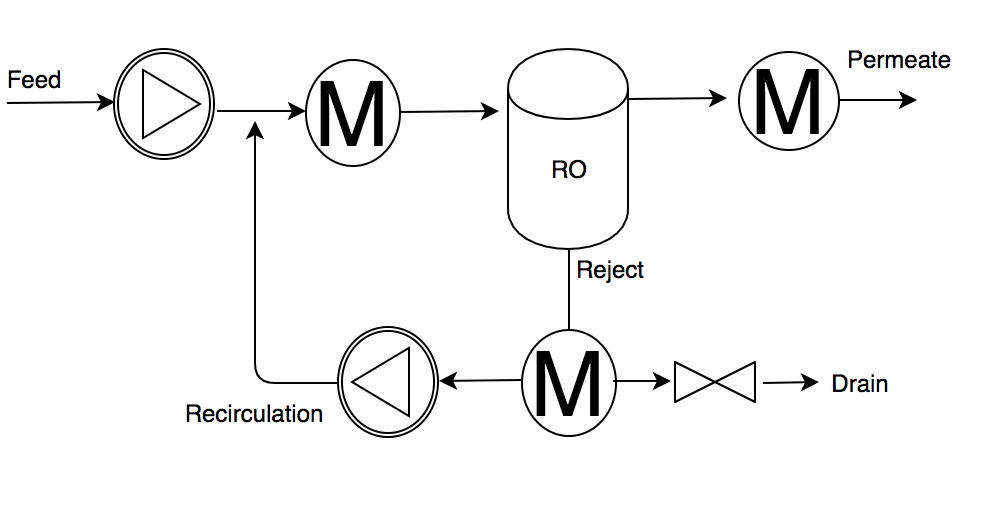
\includegraphics[width=0.7\textwidth]{MeasSys2}
    \caption{System 2, with measurement sensors}
    \label{fig:MeasSys2}
\end{figure}

\section{Test setup}
In order to compare the results from the current one pump system with the proposed two pump system, system 2, similar tests will be carried out on both systems. Measurements of interest are investigated in order to understand the how different working conditions affect the membrane. The same working conditions will be tested on both the current one pump system and on the two pump system. The critical operational areas for the membrane are considered to be high temperatures (over 30 $^\circ$C) and high conductivity (over 2000 \SI{}{\micro\siemens})/cm. The tests are performed in a range from 280-3000 \SI{}{\micro\siemens} and from 20-40 $^\circ$C. \\
\\
The working conditions that are to be investigated can be seen in Table \ref{tab:testcases}. The motor effect column is only valid for the one pump system. 


\begin{table}[H]
\centering
\begin{tabular}{|p{1.4cm}||p{2cm}|p{3.2cm}|p{1.8cm}|}
 \hline
 \textbf{Steady state }&Temperature  ($^{\circ}$C)&Feed Conductivity (\SI{}{\micro\siemens}/cm)&Motor effect (\%) \\
 \hline
 1.1 & 20 & 280  & 60 \\
 1.2 & 20 & 500  & 60 \\
 1.3 & 20 & 1000 & 60  \\
 1.4 & 20 & 1000 & \textbf{80} \\
 1.5 & 20 & 2000 & 60 \\
 1.6 & 20 & 2000 & \textbf{80}\\
 1.7 & 20 & 3000 & 60 \\
 1.8 & 20 & 3000 & \textbf{80}\\
 \hline
 2.1 & 30 & 280 & 60 \\
 2.2 & 30 & 500 & 60 \\
 2.3 & 30 & 1000 & 60 \\
 2.4 & 30 & 1000 & \textbf{80}\\
 2.5 & 30 & 2000 & 60 \\
 2.6 & 30 & 2000 & \textbf{80}\\
 2.7 & 30 & 3000 & 60 \\
 2.8 & 30 & 3000 & \textbf{80}\\
 \hline 
 3.1 & 40 & 280 & 60 \\
 3.2 & 40 & 500 & 60 \\
 3.3 & 40 & 1000 & 60 \\
 3.4 & 40 & 1000 & \textbf{80}\\
 3.5 & 40 & 2000 & 60 \\
 3.6 & 40 & 2000 & \textbf{80}\\
 3.7 & 40 & 3000 & 60 \\
 3.8 & 40 & 3000 & \textbf{80}\\
\hline
\end{tabular}
\caption{Testcases for the investigations of the membrane behaviour. Each case represents one steady state in the experiments.}
    \label{tab:testcases} 
\end{table}



%\newpage


%\section{Design of control algorithms}

%Exploratory tests on the two pump system, Figure \ref{fig:Sys2}, were executed prior the design of the control algorithms to understand how the altered flow path  pumps and drain valve. During %the tests one parameter at a time changed while the others were kept constant. In test 1, seen in Figure \ref{fig:PreTestReg1} the pump in recycle path were the changing parameter and in Test %2, seen in Figure \ref{fig:PreTestReg3} the pressurising pump on inlet side were the changing parameter. 








